%%%%%%%%%%%%%%%%%%%%%%%%%%%%%%%%%%%%%%%%%%%%%%%%%%%%%%%%%%%%%%%%%%%%%%%%%%%%%%%%%%%%%%%%%%%
%%%%%%%%%%%% Trabalho de final de curso em Eng. de Teleinformatica - UFC %%%%%%%%%%%%%%%%%%
%%%%%%%%%%%%%%%%%%%%%%%%%%%%%%%%%%%%%%%%%%%%%%%%%%%%%%%%%%%%%%%%%%%%%%%%%%%%%%%%%%%%%%%%%%%
%%%%%%%%%%%%%%%%%%%%%%%%%%%%%%%%%% Luiz Camara Neto %%%%%%%%%%%%%%%%%%%%%%%%%%%%%%%%%%%%%%%
%%%%%%%%%%%%%%%%%%%%%%%%%%%%%%%%%%%%%%%%%%%%%%%%%%%%%%%%%%%%%%%%%%%%%%%%%%%%%%%%%%%%%%%%%%%
%%%%%%%%%%%%%%%%%%%%%%%%%%%%%%% Metricas de Avaliacao %%%%%%%%%%%%%%%%%%%%%%%%%%%%%%%%%%%%
%%%%%%%%%%%%%%%%%%%%%%%%%%%%%%%%%%%%%%%%%%%%%%%%%%%%%%%%%%%%%%%%%%%%%%%%%%%%%%%%%%%%%%%%%%%

\chapter{O Sistema}
\thispagestyle{empty}

O aumento do uso de sistemas computadorizados de segmenta\c{c}\~{a}o exp\~{o}e a necessidade da proposi\c{c}\~{a}o e uso de medidas capazes de melhor avaliar a precis\~{a}o das imagens segmentadas. Neste cap\'{i}tulo, ser\'{a} apresentada uma vis\~{a}o geral da import\^{a}ncia da escolha das medidas para uma correta avalia\c{c}\~{a}o. Al\'{e}m disso, ser\~{a}o apresentadas as medidas utilizadas na abordagem de avalia\c{c}\~{a}o adotada neste trabalho.

\section{A Import\^{a}ncia das Medidas de Avalia\c{c}\~{a}o}

A avalia\c{c}\~{a}o  de desempenho \'{e} uma etapa crucial no processo de proposi\c{c}\~{a}o de um m\'{e}todo de segmenta\c{c}\~{a}o, pois somente ap\'{o}s a avalia\c{c}\~{a}o \'{e} poss\'{i}vel posicionar e comparar o novo m\'{e}todo com rela\c{c}\~{a}o a outros  dispon\'{i}veis na literatura. Para estabelecer esta compara\c{c}\~{a}o, \'{e} necess\'{a}ria a defini\c{c}\~{a}o de um crit\'{e}rio comparativo unificado que seja utilizado para ranquear os m\'{e}todos. Este crit\'{e}rio \'{e} chamado de medida de avalia\c{c}\~{a}o. Estas medidas analisam a concord\^{a}ncia entre atributos de objetos de interesse na imagem segmentada em rela\c{c}\~{a}o ao mesmo objeto em uma imagem de refer\^{e}ncia, resultando em uma informa\c{c}\~{a}o textual ou num\'{e}rica que pode ser usada para compara\c{c}\~{a}o. Atributos de \'{a}rea, di\^{a}metro, quantidade de pixels, quando corretamente segmentados, s\~{a}o exemplos que podem ser analisados por essas medidas.

A escolha das medidas usadas para avaliar o m\'{e}todo \'{e} muito importante, pois deve-se escolher medidas que analisem os atributos que melhor reflitam os objetivos principais do m\'{e}todo. Por exemplo, uma aplica\c{c}\~{a}o de detec\c{c}\~{a}o de bordas de n\'{u}cleos celulares deve dar mais import\^{a}ncia a medidas que analisem \'{a}reas e contornos do que medidas que analise a quantidade de pixels segmentados erroneamente. Neste trabalho, s\~{a}o escolhidas seis medidas de avalia\c{c}\~{a}o divididas em dois grupos, a saber, medidas de informa\c{c}\~{a}o  quantitativa e medidas de avalia\c{c}\~{a}o morfol\'{o}gica. As medidas escolhidas para a composi\c{c}\~{a}o de cada grupo foram  selecionadas com objetivo de conferir maior confiabilidade dos resultados da avalia\c{c}\~{a}o de vasos. As pr\'{o}ximas se\c{c}\~{o}es detalharam as caracter\'{i}sticas de cada grupo, as medidas usadas e suas formula\c{c}\~{o}es matem\'{a}ticas.

Neste trabalho, as imagens de refer\^{e}ncia utilizadas ser\~{a}o as imagens manualmente segmentadas por especialistas dispon\'{i}veis nas bases de imagens utilizadas. Estas imagens s\~{a}o conhecidas como mapas de refer\^{e}ncia. Para este trabalho, apenas as imagens segmentadas pelo primeiro especialista ser\~{a}o utilizadas.

\section{Medidas de Informa\c{c}\~{a}o Quantitativa}

Tr\^{e}s medidas de informa\c{c}\~{a}o quantitativas ser\~{a}o usadas neste trabalho: sensibilidade ($Sb$), especificidade ($Ep$) e precis\~{a}o ($Pc$). Estas medidas foram escolhidas por serem amplamente utilizadas por m\'{e}todos da literatura. Al\'{e}m disso, este conjunto de medidas \'{e} capaz de avaliar as taxas de acerto de cada classe segmentada individualmente, assim como a taxa de acerto global da imagem segmentada. A sensibilidade mede a taxa de acerto na segmenta\c{c}\~{a}o dos pixels de vasos sangu\'{i}neos (classe dos pixels brancos). A especificidade mede a taxa de acerto na identifica\c{c}\~{a}o de pixels n\~{a}o pertencentes a vasos sangu\'{i}neos (classe dos pixels pretos). A precis\~{a}o mede a taxa de acerto total considerando as duas classes de pixels.

\begin{figure}[!h]
    \centering
    \subfigure[\label{Fig:maskrgb}]
        {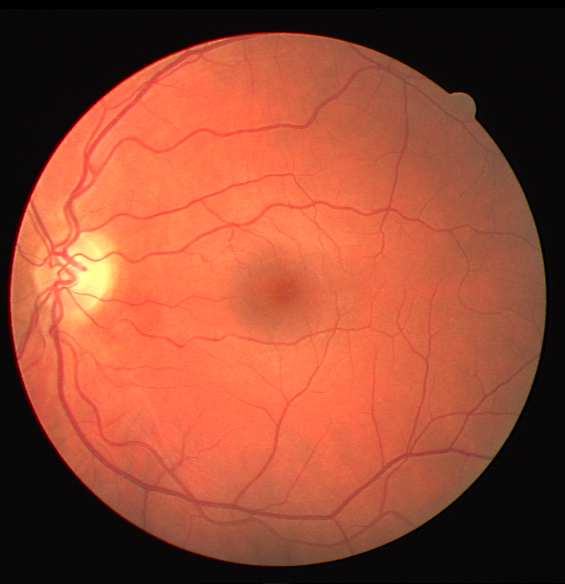
\includegraphics[width=5cm]{Figuras/Cap3/ImageRGB11}}
    \subfigure[\label{Fig:mask}]
        {
\includegraphics[width=5cm]{Figuras/Cap3/MaskDone11}}
    \caption{(a) Imagem original (Fonte: Base de dados DRIVE); (b) Imagem de m\'{a}scara (Fonte: Pr\'{o}prio Autor).}
    \label{Fig:mascara}
\end{figure}

\begin{figure}[!h]
    \centering
    \subfigure[\label{Fig:imgsegex}]
        {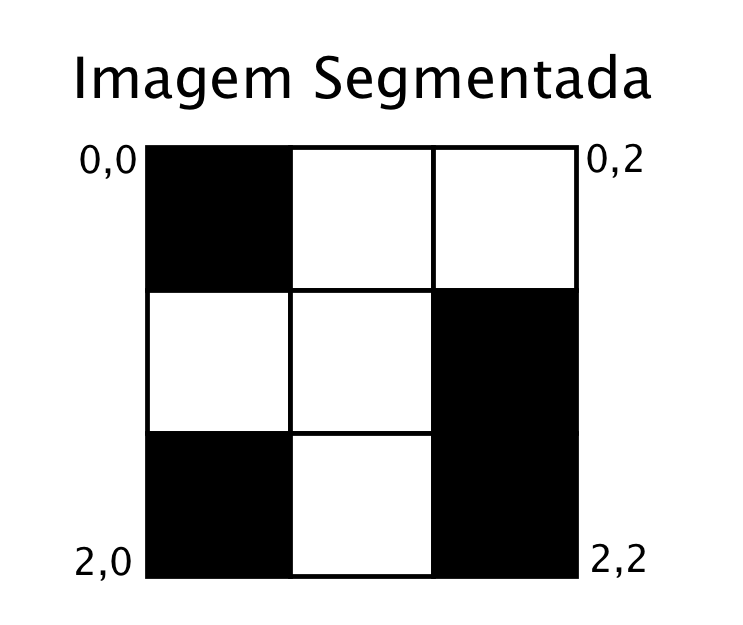
\includegraphics[width=5cm]{Figuras/Cap3/ImgSeg_ex}}
    \subfigure[\label{Fig:imgrefex}]
        {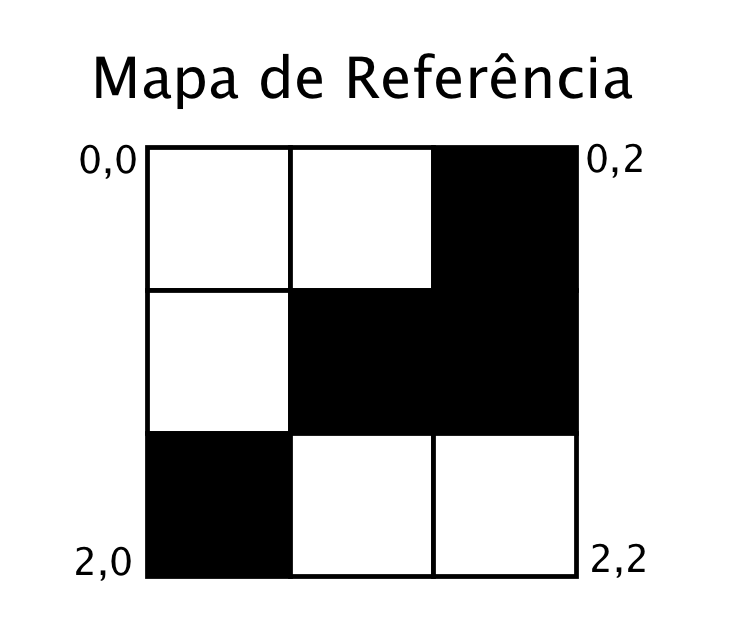
\includegraphics[width=5cm]{Figuras/Cap3/ImgRef_ex}}
    \subfigure[\label{Fig:imgresex}]
        {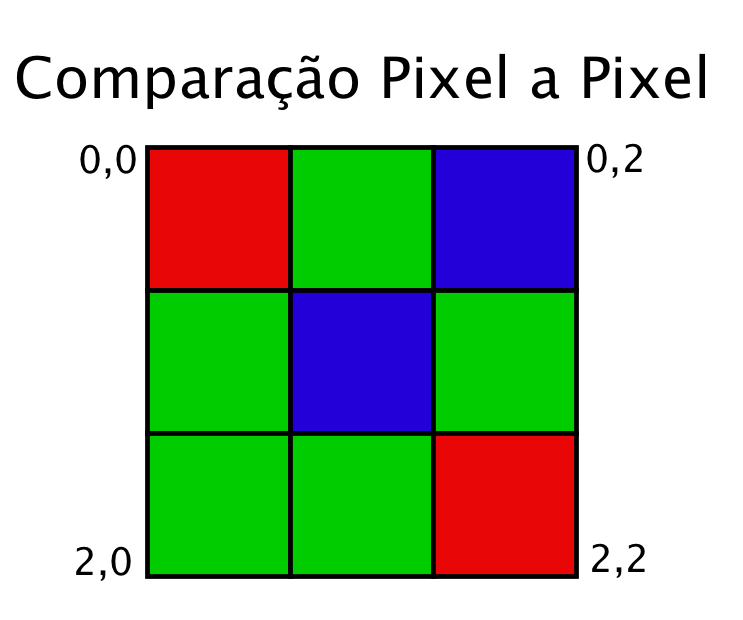
\includegraphics[width=5cm]{Figuras/Cap3/ImgRes_ex}}\\
    \caption{(a) Ilustra\c{c}\~{a}o de imagem segmentada (Fonte: Pr\'{o}prio Autor); (b) Ilustra\c{c}\~{a}o de imagem de refer\^{e}ncia (Fonte: Pr\'{o}prio Autor); (c) Resultado de avalia\c{c}\~{a}o pixel a pixel (Fonte: Pr\'{o}prio Autor).}
    \label{Fig:exemples}
\end{figure}

O c\'{a}lculo utilizado para determina\c{c}\~{a}o num\'{e}rica destas medidas baseia-se na contagem de pixels correspondentes entre a imagem segmentada e o mapa de refer\^{e}ncia. Contudo, apenas os pixels localizados externamente ao campo de vis\~{a}o s\~{a}o considerados para c\'{a}lculo. Para isto, uma imagem de m\'{a}scara \'{e} utilizada para isolar os pixels que devem ser contabilizados como ilustrado na Figura \ref{Fig:mascara}. A Figura \ref{Fig:exemples} ilustra uma avalia\c{c}\~{a}o de correspond\^{e}ncia pixel a pixel para uma imagem de tamanho $3\times3$ pixels. As Figuras \ref{Fig:imgsegex} e \ref{Fig:imgrefex} mostram exemplos de uma imagem segmentada e seu mapa de refer\^{e}ncia associado, respectivamente. O resultado da avalia\c{c}\~{a}o pode ser visto na Figura \ref{Fig:imgresex}. Os pixels vermelhos e azuls ilustram erros na detec\c{c}\~{a}o  de pixels brancos e pretos, respectivamente. Cada pixel vermelho indica um pixel preto onde deveria estar um pixel branco. Em contrapartida, cada pixel azul indica um pixel branco onde deveria estar um pixel preto. Os pixels verdes ilustram as posi\c{c}\~{o}es com valores coincidentes. Ao final \'{e} poss\'{i}vel calcular as taxas de acerto e erro para cada classe, bem como para a imagem completa. Este padr\~{a}o de cores ser\'{a} usado para compara\c{c}\~{a}o ao longo de todo este trabalho. As equa\c{c}\~{o}es abaixo mostram as formula\c{c}\~{o}es matem\'{a}ticas para o c\'{a}lculo da sensibilidade ($Sb$), especificidade ($Ep$) e precis\~{a}o ($Pc$), respectivamente.

\begin{equation}
Sb = \frac{VP}{VP + FN},
\end{equation}

\begin{equation}
Ep = \frac{VN}{VN + FP},
\end{equation}

\begin{equation}\label{eq:acuracia}
Pc = \frac{VP + VN}{VP + VN + FP + FN},
\end{equation}

\noindent uma vez que $VP$, $VN$, $FP$ e $FN$ representam o n\'{u}mero de acertos de pixels de vasos, o n\'{u}mero de acertos de pixels n\~{a}o pertencentes aos vasos, o n\'{u}mero de pixels segmentados erroneamente como vasos e o n\'{u}mero de pixels, erroneamente segmentados, como n\~{a}o pertencentes aos vasos, respectivamente. A Tabela \ref{tabNotacao} ilustra a rela\c{c}\~{a}o de correspond\^{e}ncia entre os pixels da imagem segmentada e os pixels do mapa de refer\^{e}ncia para determina\c{c}\~{a}o dos elementos formadores das medidas.

  \begin{table}[h]
    \caption{Ilustra\c{c}\~{a}o da nota\c{c}\~{a}o de correspond\^{e}ncia entre a imagem segmentada e o mapa de refer\^{e}ncia.}
    \label{tabNotacao}
    \centering
    \scalebox {0.85 }[0.85 ]{ 
      \begin{tabular}{c|cccc}
        \toprule
        Nota\c{c}\~{a}o & Imagem Segmentada & Mapa de Refer\^{e}ncia \\
        \midrule                 
        $VP$  &\textbf{Vaso} &\textbf{Vaso} \\
        $VN$  &N\~{a}o-Vaso &N\~{a}o-Vaso \\
        $FP$  &\textbf{Vaso} &N\~{a}o-Vaso \\
        $FN$  &N\~{a}o-Vaso &\textbf{Vaso} \\
        \bottomrule
      \end{tabular}
    }
  \end{table}

Apesar de serem amplamente utilizadas como \'{u}nicas medidas de avalia\c{c}\~{a}o, as medidas quantitativas n\~{a}o s\~{a}o capazes de determinar o desempenho dos m\'{e}todos de maneira satisfat\'{o}ria. Como citado anteriormente, atributos relevantes n\~{a}o s\~{a}o levados em considera\c{c}\~{a}o por estas medidas. Por isso, este trabalho prop\~{o}e que estas medidas sejam utilizadas em conjunto com outras que analisem atributos morfol\'{o}gicos relevantes da rede segmentada, como conectividade, \'{a}rea e comprimento dos vasos. 

\section{Medidas de Avalia\c{c}\~{a}o Morfol\'{o}gica}

Medidas de determina\c{c}\~{a}o da taxa de acerto de classes baseada na contagem de coincid\^{e}ncia pixel a pixel n\~{a}o s\~{a}o suficientes para precisar satisfatoriamente o desempenho do m\'{e}todo sob avalia\c{c}\~{a}o, pois estas medidas n\~{a}o cont\^{e}m informa\c{c}\~{a}o qualitativa em seus resultados. Informa\c{c}\~{o}es qualitativas s\~{a}o importantes quando avaliamos uma segmenta\c{c}\~{a}o, pois elas s\~{a}o capazes de analisar a semelhan\c{c}a da imagem segmentada com o mapa de refer\^{e}ncia em rela\c{c}\~{a}o a um atributo espec\'{i}fico do objeto de interesse da imagem. Por exemplo, medidas que analisam \'{a}rea, di\^{a}metro, largura de objetos cont\^{e}m informa\c{c}\~{a}o sobre o grau de semelhan\c{c}a entre estes objetos na imagem segmentada e os respectivos objetos no mapa de refer\^{e}ncia em rela\c{c}\~{a}o \`{a} \'{a}rea, di\^{a}metro e largura, respectivamente. Portanto, medidas qualitativas s\~{a}o usadas como complementares das medidas quantitativas na  avalia\c{c}\~{a}o para fornecer uma an\'{a}lise destacada dos atributos relevantes a serem avaliados.

Para este trabalho as medidas qualitativas para avalia\c{c}\~{a}o morfol\'{o}gica ser\~{a}o respons\'{a}veis pela avalia\c{c}\~{a}o de tr\^{e}s atributos estruturais da rede segmentada usados para diversas aplicac\~{o}es. Por isso, estas medidas ser\~{a}o referidas como medidas de avalia\c{c}\~{a}o morfol\'{o}gica. Estas medidas, adotadas neste trabalho, foram introduzidas em \citeauthor{Gegundez2013} (\citeyear{Gegundez2013}) para avaliar a conectividade, a \'{a}rea e o comprimento dos elemetos na imagem segmentada. As medidas s\~{a}o hom\^onimas aos atributos avaliados e s\~{a}o referidas por conectividade ($C$), \'{a}rea ($A$) e comprimento ($L$). A conectividade avalia o grau de fragmenta\c{c}\~{a}o da rede de vasos entre a imagem segmentada e o mapa de refer\^{e}ncia. A \'{a}rea avalia o grau de sobreposi\c{c}\~{a}o das \'{a}reas dos vasos entre a imagem segmentada e o mapa de refer\^{e}ncia. O comprimento avalia o grau de similaridade dos comprimentos totais da rede de vasos na imagem segmentada e no mapa de refer\^{e}ncia. Assumindo a imagem segmentada e o mapa de refer\^{e}ncia por $I_{sg}$ e $I_{mr}$, as f\'{o}rmulas para determina\c{c}\~{a}o destas medidas s\~{a}o mostradas abaixo. 

\begin{equation}
C = 1 - min\left( 1, \frac{|\#_c(I_{mr}) - \#_c(I_{sg})|}{\#(I_{mr})} \right),
\end{equation}

\begin{equation}
A = \frac{\#((\delta(I_{sg}) \cap I_{mr}) \cup (I_{sg} \cap \delta(I_{mr})))}{\#(I_{sg} \cup I_{mr})},
\end{equation}

\begin{equation}
L = \frac{\#((\varphi(I_{sg}) \cap \delta(I_{mr})) \cup (\delta(I_{sg}) \cap \varphi(I_{mr})))}{\#(\varphi(I_{sg}) \cup \varphi(I_{mr}))},
\end{equation}

\noindent onde $min$, $\#_c()$ e $\#$ s\~{a}o as fun\c{c}\~{o}es de determina\c{c}\~{a}o do m\'{i}nimo valor, do n\'{u}mero de componentes conectados e da cardinalidade do conjunto, respectivamente. $\delta()$ e $\varphi()$ s\~{a}o os operadores morfol\'{o}gicos de dilata\c{c}\~{a}o usando um disco de tr\^{e}s pixels e de esqueletiza\c{c}\~{a}o homot\'{o}pica \cite{Soille:2003}, respectivamente. Portanto, a abordagem proposta avalia a qualidade da segmenta\c{c}\~{a}o com medidas quantitativas. Essa abordagem tamb\'{e}m aplica as medidas de avalia\c{c}\~{a}o morfol\'{o}gica para que possamos ter uma an\'{a}lise completa do desempenho do m\'{e}todo em fun\c{c}\~{a}o das taxas de acerto e dos atributos relevantes da rede segmentada. 

\section{Considera\c{c}\~{o}es Finais}

Neste cap\'{i}tulo foi apresentado o conjunto das medidas de avalia\c{c}\~{a}o que ser\'{a} usado para avaliar os m\'{e}todos na nova abordagem. Este conjunto foi composto baseado na complementaridade de informa\c{c}\~{a}o entre os dois grupos de medidas, o que permite tornar a avalia\c{c}\~{a}o mais robusta e confi\'{a}vel. Al\'{e}m diso, foi discutido a import\^{a}ncia da escolha das medidas para obten\c{c}\~{a}o de uma avalia\c{c}\~{a}o mais precisa.

No pr\'{o}ximo cap\'{i}tulo ser\~{a}o apresentados e discutidos os resultados obtidos a partir da aplica\c{c}\~{a}o da abordagem proposta nas imagens segmentadas pelos m\'{e}todos detalhados no cap\'{i}tulo anterior.